\renewcommand{\theequation}{\theenumi}
\renewcommand{\thefigure}{\theenumi}
\begin{enumerate}[label=\thesubsection.\arabic*.,ref=\thesubsection.\theenumi]
\numberwithin{equation}{enumi}
\numberwithin{figure}{enumi}

\item Find the distance between the following pair of points
(11,16) and (23,21).\\
Let 
\begin{align}
    \vec{A} = \myvec{11\\16}, \vec{B} = \myvec{23\\21}
\end{align}
Then,
\begin{align}
\vec{B}-\vec{A} = \myvec{12\\5}\;
\end{align}
and
%
\begin{align}
 \norm{\vec{B}-\vec{A}}^2= (\vec{B}-\vec{A})^\top (\vec{B}-\vec{A})\;
&=  \myvec{12 \ 5} \myvec{12\\5}\\
\implies \norm{\vec{B}-\vec{A}}&=\sqrt{(12^2 + 5^2)}\\\nonumber
&=13\\\nonumber
\end{align}



\item Find the distance between the following pair of points
(66,25) and (99,69).
\\
Let
\begin{align}
    \vec{A} = \myvec{66\\25}, \vec{B} = \myvec{99\\69}
\end{align}
Then
\begin{align}
\norm{\vec{B}-\vec{A}}=\norm{\vec {C}}
\end{align}
\begin{align}
 \norm{\vec{C}}^2 &= \vec{C}^\top \vec{C} \\
&=  \myvec{33 \ 44} \myvec{33\\44}\\
\implies \norm{\vec{C}}=\sqrt{(33^2 + 44^2)}\\
&=55
\end{align}
%
\item Find the distance between the following pairs of points  with the axes at 60\degree
\begin{enumerate}
    \item \myvec{7\\6} and \myvec{4\\5}
    \solution
    
Let the given points in the angular axis be
\begin{equation}
\myvec{x_1\\y_1} = \ \myvec{4 \\5} \ ; \ \myvec{x_2\\y_2} \ = \myvec{7\\ 6}\label{2/solution/2/11.0.1}
\end{equation}
From    Fig. \ref{2/solution/2/1Fig1: Points plotted in Python},
the corresponding points in the rectangular axis are
\begin{align}
x_3 = x_1+y_1\cos 60\degree\\
y_3 = y_1\cos 30\degree
% \end{align}
% In order to convert to rectangular coordinate system, the y-axis should be rotated by $30\degree$ in anti-clockwise.
% Transformed coordinates of \myvec{x_1\\y_1} \& \myvec{x_2\\y_2} be \myvec{x_3\\y_3} \& \myvec{x_4\\y_4} respectively.
% \begin{equation}
\implies \myvec{x_3\\y_3} = \myvec{1 \ \cos{60\degree} \\ 0 \  \cos{30\degree}} \myvec{x_1\\y_1}\label{2/solution/2/1eq:1.0.2}   
\end{align}
% \end{equation}
Similarly,\\
\begin{align}
    \myvec{x_4\\y_4} = \myvec{1 \ \cos{60\degree} \\ 0 \  \cos{30\degree}} \myvec{x_2\\y_2}\label{2/solution/2/1eq:1.0.3}
\end{align}
    
% $x_4$ = O$X_2$ + $X_2$$X_4$ = $x_2$+$y_2$\cos{60\degree$$ \\
% $y_4$ = O$Y_2$$\cos{30\degree$$  =\ $y_2$$\cos{30\degree$\\
% \begin{equation}
% \end{equation}
In general, the rectangular coordinates can be express in terms of the angular coordinates through the 
linear transformation
\begin{equation}
    \vec{x}_r &= \vec{P}\vec{x}, \\
    \text{where, }
vec{P}&= \myvec{1   &  \cos \theta \\ 0 & \sin \theta} 
\end{equation}
Thus, the distance between two points $\vec{x}_1, \vec{x}_2$ in the angular axis  is given by
\begin{align}
    \norm{\vec{P}\brak{\vec{x}_1-\vec{x}_2}} &= \sqrt{\brak{\vec{x}_1-\vec{x}_2}^\top\vec{P}^\top \vec{P}\brak{\vec{x}_1-\vec{x}_2}} \\
    &= \sqrt{13}
\end{align}


% Substituting \eqref{2/solution/2/11.0.1} in \eqref{2/solution/2/1eq:1.0.2} \& \eqref{2/solution/2/1eq:1.0.3}
%  \begin{equation}
%   \myvec{x_3\\y_3} = \myvec{\frac{13}{2}\\\frac{5\sqrt{3}}{2}};\ \myvec{x_4\\y_4} = \myvec{10\\3\sqrt{3}}\label{2/solution/2/1eq:1.0.5}    
%  \end{equation}
% The distance between points is a norm of the distance vector,\\ \norm{\myvec{x_3\\y_3} - \myvec{x_4\\y_4}} = \norm{\myvec{10\\3\sqrt{3}} - \myvec{\frac{13}{2}\\\frac{5\sqrt{3}}{2}}} = 
%  $ \  \sqrt{13} \  units$\\ \\
%  The distance, d can be measured in angular axes directly by following equation,
%  \begin{align}
%  d = \sqrt{{\norm{\myvec{x_2\\y_2} - \myvec{x_1\\y_1}}}^2 +2\myvec{x_2-x_1\\0}^\top \myvec{y_2-y_1\\0}\cos{\theta}}\\ 
% d = \sqrt{{\norm{\myvec{7\\6} - \myvec{4\\5}}}^2 +2\myvec{3&0} \myvec{1\\0}\cos{60\degree}} 
% \end{align}
% \begin{align}
% d = \sqrt{13} \ units    
%  \end{align}
%  \\
% Above results shows that the distance remains constant between the points irrespective of coordinate system and by \eqref{2/solution/2/11.0.1} \& \eqref{2/solution/2/1eq:1.0.5} only the position vector of the point changes with the transformation of coordinate system\\ \\ 
\begin{figure}[!ht]
	\centering
	\includegraphics[width=\columnwidth]{2/solution/2/1fig1.png}
	\caption{Points defined on angular \& rectangular axes}
    \label{2/solution/2/1Fig1: Points plotted in Python}

	\end{figure}
	
% \counterwithin{figure}{section}
% \begin{figure}[!ht]
%     \centering
%     \includegraphics[width=\columnwidth]{2/solution/2/1download.png}
%     \caption{Points plotted in Python}
%     \label{2/solution/2/1Fig2: Points plotted in Python}
% \end{figure}

\end{enumerate}
\item Find the area of the quadrilateral formed by the points
\begin{enumerate}
\item 
\begin{align}
\begin{split}
\vec{A} = \myvec{1 \\ 1}, 
\vec{B} = \myvec{3 \\ 5}, 
\vec{C} = \myvec{-2 \\ 4}, 
\vec{D} = \myvec{-1 \\ -5}.
\end{split}
\end{align}
\solution
Let 
\begin{align}
\begin{split}
\vec{A} = \myvec{1 \\ 1}, 
\vec{B} = \myvec{3 \\ 5}, 
\vec{C} = \myvec{-2 \\ 4}, 
\vec{D} = \myvec{-1 \\ -5}. 
\end{split}
\end{align}
Then, 
\begin{align}
\brak{\vec{B} - \vec{A}}
    &= \myvec{3\\5} - \myvec{1\\1}
    = \myvec{2\\4}
\\
    \brak{\vec{D} - \vec{B}}
    &= \myvec{-1\\-5} - \myvec{3\\5}
    = \myvec{-4\\-10}
\\
     \brak{\vec{A} - \vec{D}}
    &= \myvec{1\\1} - \myvec{-1\\-5}
    = \myvec{2\\6}
\end{align}
%
Row reducing the matrix formed by the  vectors, 
\begin{align}
%\begin{math}
\myvec{2 & 4 & 1\\-4 & -10 & 1\\2 & 6 & 1\\}
\\
\implies 
\myvec{2 & 4 & 1\\-4 & -10 & 1\\2 & 6 & 1\\}
\xleftrightarrow[]{R_2\leftrightarrow R_3}
\myvec{2 & 4 & 1\\2 & 6 & 1\\-4 & -10 & 1\\}
\xleftrightarrow[]{R_3\leftrightarrow R_1+R_2+R_3}
\myvec{2 & 4 & 1\\2 & 6 & 1\\0 & 0 & 3\\}
\xleftrightarrow[]{R_2\leftrightarrow R_2-R_1}
\myvec{2 & 4 & 1\\0 & 2 & 0\\0 & 0 & 3\\}
%\end{math}
\end{align}
The number of non-zero rows in the matrix = 3. Hence the matrix
is full rank and  AB, BD, DA are not collinear.
See Fig. \ref{hem/2/9/1/fig:Quad ABCD}, which shows that the points given form a quadrilateral.
\begin{figure}[!ht]
    \centering
    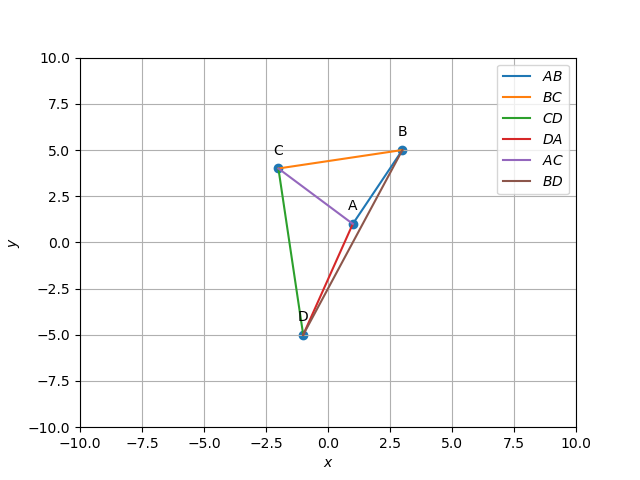
\includegraphics[width=\columnwidth]{2/solution/9/1/QUAD.png}
    \caption{Quadrilateral ABCD}
    \label{hem/2/9/1/fig:Quad ABCD}
\end{figure}
%
Area of a $\triangle ABC$ is given by
%
\begin{align}
\triangle ABC = 
\frac{1}{2}\mydet{
1 & 1 & 1\\1 & 3 & -2\\1 & 5 & 4\\}
= 9
\end{align}
%
Area of $\triangle ACD$  is given by
\begin{align}
\triangle ACD = 
\frac{1}{2}\mydet{
1 & 1 & 1\\1 & -2 & -1\\1 & 4 & -5\\}
= 11.5
\end{align}
Thus, the area of quadrilateral ABCD = 9+11.5 = 20.5.

\item 
\begin{align}
\vec{P} = \myvec{2\\1}, \vec{Q} =\myvec{3\\5},
\vec{R} =\myvec{-3\\4}, \vec{S} =\myvec{-2\\-2}
\end{align}
\solution

In Fig.     \ref{2/9/2fig:Quad PQRS},
 Area of a Quadrilateral PQRS=
\begin{align}
Area (\triangle PQR)+ Area (\triangle PRS)=
\end{align}
\begin{equation}
\frac{1}{2}\norm{(\vec{Q}-\vec{P})\times(\vec{Q}-\vec{R})}+\frac{1}{2}\norm{\mathbf{(\vec{S}-\vec{P})\times(\vec{S}-\vec{R})}}
\label{2/9/2eq:1}
\end{equation}
For two vectors
\begin{align}
\vec{a}=\myvec{a_1\\a_2} , \vec{b}=\myvec{b_1\\b_2}
\end{align}
\begin{equation}
\norm{\mathbf{\vec{a}\times\vec{b}}}=\abs{(a_1b_2-a_2b_1)}
\label{2/9/2eq:2}
\end{equation}
\begin{align}
\vec{Q-P}=\myvec{1\\4}\\
\vec{Q-R}=\myvec{6\\1}\\
\vec{S-P}=\myvec{-4\\-3}\\
\vec{S-R}=\myvec{1\\-6}
\end{align}
Using equation \eqref{2/9/2eq:2}
\begin{equation}
\frac{1}{2}\norm{\mathbf{(\vec{Q}-\vec{P})\times(\vec{Q}-\vec{R})}}
=\frac{1}{2}\abs{(-23)}=11.5
\label{2/9/2eq:3}
\end{equation}
\begin{equation}
\frac{1}{2}\norm{\mathbf{(\vec{S}-\vec{P})\times(\vec{S}-\vec{R})}}
=\frac{1}{2}\abs{(27)}=13.5    
\label{2/9/2eq:4}
\end{equation}
Substituting values from equation \eqref{2/9/2eq:3} and \eqref{2/9/2eq:4} in equation \eqref{2/9/2eq:1},the desired area is
\begin{align}
11.5+13.5
=25 
\end{align}
\begin{figure}[!ht]
    \centering
    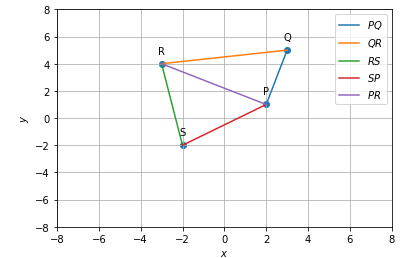
\includegraphics[width=\columnwidth]{2/solution/2/9/2/QUAD.PNG}
    \caption{Quadrilateral PQRS}
    \label{2/9/2fig:Quad PQRS}
\end{figure}




\end{enumerate}
\end{enumerate}
